\documentclass[14pt]{extbook}
\usepackage{multicol, enumerate, enumitem, hyperref, color, soul, setspace, parskip, fancyhdr} %General Packages
\usepackage{amssymb, amsthm, amsmath, latexsym, units, mathtools} %Math Packages
\everymath{\displaystyle} %All math in Display Style
% Packages with additional options
\usepackage[headsep=0.5cm,headheight=12pt, left=1 in,right= 1 in,top= 1 in,bottom= 1 in]{geometry}
\usepackage[usenames,dvipsnames]{xcolor}
\usepackage{dashrule}  % Package to use the command below to create lines between items
\newcommand{\litem}[1]{\item#1\hspace*{-1cm}\rule{\textwidth}{0.4pt}}
\pagestyle{fancy}
\lhead{Progress Quiz 10}
\chead{}
\rhead{Version C}
\lfoot{1995-1928}
\cfoot{}
\rfoot{test}
\begin{document}

\begin{enumerate}
\litem{
Solve the equation below. Then, choose the interval that contains the solution.\[ -11(-9x -19) = -13(5x -8) \]\begin{enumerate}[label=\Alph*.]
\item \( x \in [1, 2] \)
\item \( x \in [-2.9, -0.7] \)
\item \( x \in [-1, 0.1] \)
\item \( x \in [-9.6, -8.9] \)
\item \( \text{There are no real solutions.} \)

\end{enumerate} }
\litem{
Solve the linear equation below. Then, choose the interval that contains the solution.\[ \frac{4x -9}{8} - \frac{3x + 7}{5} = \frac{3x -3}{4} \]\begin{enumerate}[label=\Alph*.]
\item \( x \in [-0.4, 2] \)
\item \( x \in [-15.4, -13.7] \)
\item \( x \in [-1.9, -0.1] \)
\item \( x \in [-2.6, -2] \)
\item \( \text{There are no real solutions.} \)

\end{enumerate} }
\litem{
Find the equation of the line described below. Write the linear equation as $ y=mx+b $ and choose the intervals that contain $m$ and $b$.\[ \text{Parallel to } 9 x + 7 y = 6 \text{ and passing through the point } (-7, -7). \]\begin{enumerate}[label=\Alph*.]
\item \( m \in [-2.13, -1.25] \hspace*{3mm} b \in [-17.7, -15.5] \)
\item \( m \in [-2.13, -1.25] \hspace*{3mm} b \in [-1.3, 0.5] \)
\item \( m \in [-1.05, -0.64] \hspace*{3mm} b \in [-17.7, -15.5] \)
\item \( m \in [1.24, 1.65] \hspace*{3mm} b \in [1.7, 5.3] \)
\item \( m \in [-2.13, -1.25] \hspace*{3mm} b \in [15.2, 16.2] \)

\end{enumerate} }
\litem{
First, find the equation of the line containing the two points below. Then, write the equation as $ y=mx+b $ and choose the intervals that contain $m$ and $b$.\[ (-10, -7) \text{ and } (6, -2) \]\begin{enumerate}[label=\Alph*.]
\item \( m \in [0.2, 4.9] \hspace*{3mm} b \in [-4.54, -3.33] \)
\item \( m \in [0.2, 4.9] \hspace*{3mm} b \in [3.15, 3.98] \)
\item \( m \in [-3.7, -0.1] \hspace*{3mm} b \in [-0.67, 0.5] \)
\item \( m \in [0.2, 4.9] \hspace*{3mm} b \in [-8.11, -7.45] \)
\item \( m \in [0.2, 4.9] \hspace*{3mm} b \in [2.91, 3.11] \)

\end{enumerate} }
\litem{
First, find the equation of the line containing the two points below. Then, write the equation as $ y=mx+b $ and choose the intervals that contain $m$ and $b$.\[ (9, 5) \text{ and } (-10, 10) \]\begin{enumerate}[label=\Alph*.]
\item \( m \in [0.08, 0.81] \hspace*{3mm} b \in [9.5, 14.1] \)
\item \( m \in [-0.41, -0.19] \hspace*{3mm} b \in [-9.5, -7] \)
\item \( m \in [-0.41, -0.19] \hspace*{3mm} b \in [7.2, 10.5] \)
\item \( m \in [-0.41, -0.19] \hspace*{3mm} b \in [18.4, 22.6] \)
\item \( m \in [-0.41, -0.19] \hspace*{3mm} b \in [-4.9, -1.8] \)

\end{enumerate} }
\litem{
Write the equation of the line in the graph below in Standard form $Ax+By=C$. Then, choose the intervals that contain $A, B, \text{ and } C$.
\begin{center}
    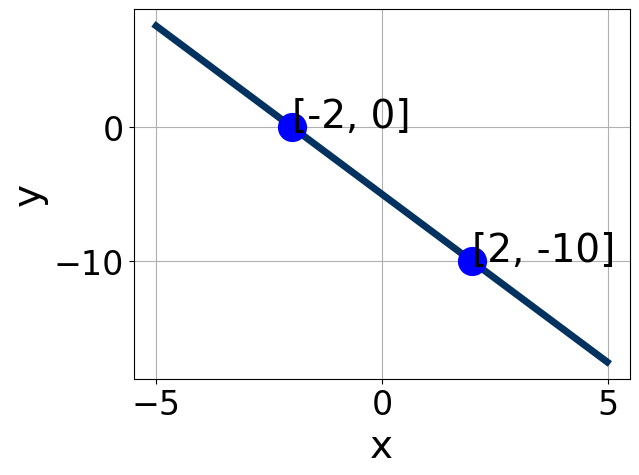
\includegraphics[width=0.5\textwidth]{../Figures/linearGraphToStandardC.png}
\end{center}
\begin{enumerate}[label=\Alph*.]
\item \( A \in [-1.25, 2.75], \hspace{3mm} B \in [-2.5, -0.3], \text{ and } \hspace{3mm} C \in [-4, 0] \)
\item \( A \in [-10, -1], \hspace{3mm} B \in [-4.8, -2.9], \text{ and } \hspace{3mm} C \in [-17, -7] \)
\item \( A \in [2, 6], \hspace{3mm} B \in [1.7, 6.4], \text{ and } \hspace{3mm} C \in [6, 15] \)
\item \( A \in [-1.25, 2.75], \hspace{3mm} B \in [0.5, 2.3], \text{ and } \hspace{3mm} C \in [-1, 6] \)
\item \( A \in [2, 6], \hspace{3mm} B \in [-4.8, -2.9], \text{ and } \hspace{3mm} C \in [-17, -7] \)

\end{enumerate} }
\litem{
Solve the linear equation below. Then, choose the interval that contains the solution.\[ \frac{9x + 9}{5} - \frac{9x -8}{4} = \frac{-7x + 4}{8} \]\begin{enumerate}[label=\Alph*.]
\item \( x \in [-2.47, 0.53] \)
\item \( x \in [-11.76, -4.76] \)
\item \( x \in [0.65, 3.65] \)
\item \( x \in [-32.59, -27.59] \)
\item \( \text{There are no real solutions.} \)

\end{enumerate} }
\litem{
Write the equation of the line in the graph below in Standard form $Ax+By=C$. Then, choose the intervals that contain $A, B, \text{ and } C$.
\begin{center}
    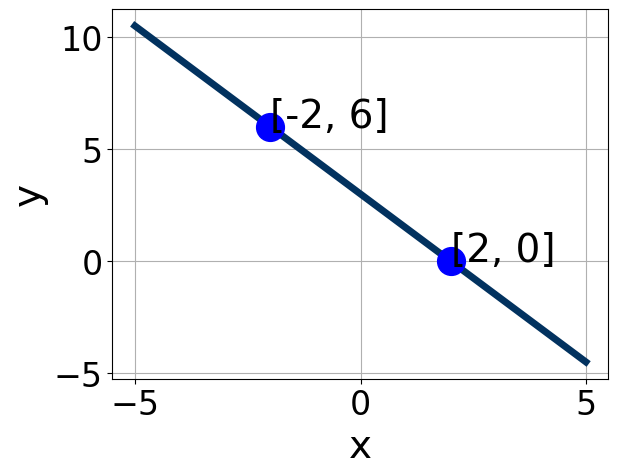
\includegraphics[width=0.5\textwidth]{../Figures/linearGraphToStandardCopyC.png}
\end{center}
\begin{enumerate}[label=\Alph*.]
\item \( A \in [-2.67, -1.99], \hspace{3mm} B \in [4.47, 6.67], \text{ and } \hspace{3mm} C \in [9, 12] \)
\item \( A \in [-1.02, 0.67], \hspace{3mm} B \in [0.56, 1.7], \text{ and } \hspace{3mm} C \in [-1, 7] \)
\item \( A \in [1.43, 2.26], \hspace{3mm} B \in [-5.01, -4.02], \text{ and } \hspace{3mm} C \in [-11, -8] \)
\item \( A \in [1.43, 2.26], \hspace{3mm} B \in [4.47, 6.67], \text{ and } \hspace{3mm} C \in [9, 12] \)
\item \( A \in [-1.02, 0.67], \hspace{3mm} B \in [-2.26, -0.01], \text{ and } \hspace{3mm} C \in [-3, 1] \)

\end{enumerate} }
\litem{
Find the equation of the line described below. Write the linear equation as $ y=mx+b $ and choose the intervals that contain $m$ and $b$.\[ \text{Perpendicular to } 5 x + 4 y = 3 \text{ and passing through the point } (-5, 2). \]\begin{enumerate}[label=\Alph*.]
\item \( m \in [0.83, 1.26] \hspace*{3mm} b \in [5.73, 6.88] \)
\item \( m \in [0.52, 0.93] \hspace*{3mm} b \in [5.73, 6.88] \)
\item \( m \in [-0.89, -0.66] \hspace*{3mm} b \in [-2.7, -1.71] \)
\item \( m \in [0.52, 0.93] \hspace*{3mm} b \in [-6.63, -5.71] \)
\item \( m \in [0.52, 0.93] \hspace*{3mm} b \in [6.97, 7.65] \)

\end{enumerate} }
\litem{
Solve the equation below. Then, choose the interval that contains the solution.\[ -12(-17x + 16) = -15(-18x -13) \]\begin{enumerate}[label=\Alph*.]
\item \( x \in [-5.88, -5.83] \)
\item \( x \in [-0.06, -0.03] \)
\item \( x \in [-0.04, 0] \)
\item \( x \in [0.04, 0.08] \)
\item \( \text{There are no real solutions.} \)

\end{enumerate} }
\end{enumerate}

\end{document}